We present the grid search space in Figure \ref{fig:cl_hp}, and report the best parameters found in 
Table \ref{tab:cl_par}. With this set of parameter the network results fully trained in only $7$ epochs.
\begin{table}[h]
    \centering
    \begin{tabular}{cccc} \hline
        Dropout & Learning rate & Optimizer & Regularization  \\ \hline
        $0.1$   & $0.003$       & Adam      & $0.001$         
    \end{tabular}
    \caption{Optimal parameters for the classification task.}
    \label{tab:cl_par}
\end{table}
We can see that the regularization, through both the dropout and the L2 regularization, is higher in this case, meaning that this 
task requires particular attention to avoid overfitting.

The accuracy on the test set of the model gave optimal results, with an accuracy of $0.999$.

We present in Figure \ref{fig:cl_f1} the filters of the first convolutional layer and in 
Figure \ref{fig:cl_f2} the filters of the second convolutional layer. They are, however, of difficult interpretation. We can 
however see in Figure \ref{fig:cl_f2} a pattern that suggests that these filters are looking for edges in the figures.
\begin{figure}[h]
    \centering
    \begin{minipage}[t]{0.48\textwidth}
        \centering
        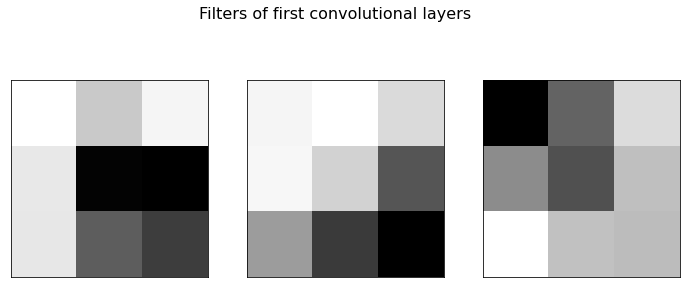
\includegraphics[width=0.98\textwidth]{Images/clas_filt1.png}
        \caption{$3\times3$ kernels of the filters of the first convolutional layer. It is not particularly clear which are
        the enhanced features. }
        \label{fig:cl_f1}
    \end{minipage}\hfill
    \begin{minipage}[t]{0.48\textwidth}
        \centering
        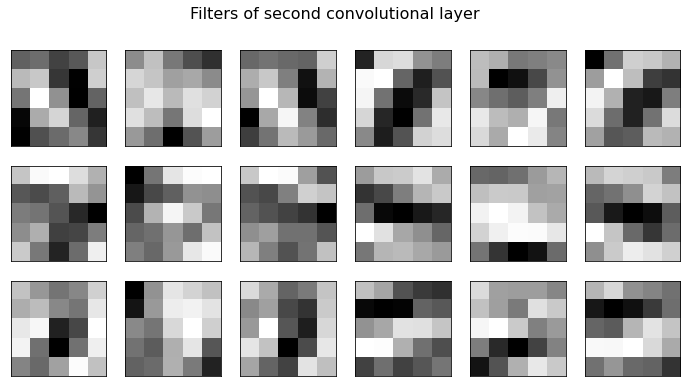
\includegraphics[width=0.98\textwidth]{Images/clas_filt2.png}
        \caption{$5\times5$ kernels of the filters of the second convolutional layer. We can observe black lines, which correspond
        to an enhancement of the edges.}
        \label{fig:cl_f2}
    \end{minipage}
\end{figure}

It is more interesting to analyze the activation profiles of the convolutional layers. In Figure \ref{fig:cl_a1} we can 
observe in a really clear way the digit that was given in input, while in \ref{fig:cl_a2} we can observe the enhancement 
of the edges of that number, as suggested by the filter.
\begin{figure}[h]
    \centering
    \begin{minipage}[t]{0.48\textwidth}
        \centering
        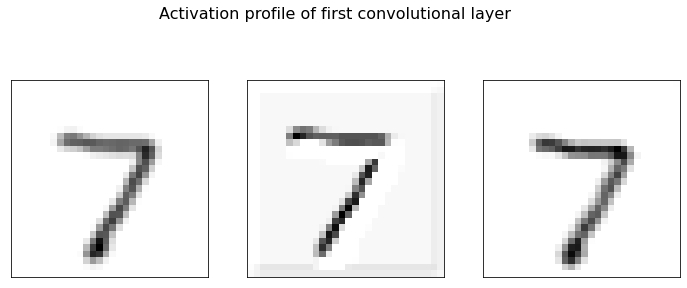
\includegraphics[width=0.98\textwidth]{Images/clas_act1.png}
        \caption{The three channels in output from the first convolutional layer. We can observe the input digit, which is a
        $7$. }
        \label{fig:cl_a1}
    \end{minipage}\hfill
    \begin{minipage}[t]{0.48\textwidth}
        \centering
        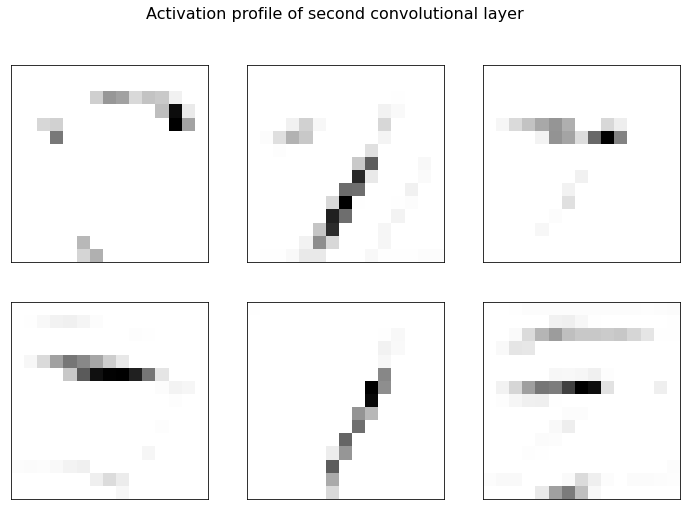
\includegraphics[width=0.98\textwidth]{Images/clas_act2.png}
        \caption{The six channels in output from the second convolutional layer. We can observe a decomposition of the input 
        digit in edges, which is common in convolutional networks. }
        \label{fig:cl_a2}
    \end{minipage}
\end{figure}